\chapter{緒論}

\section{研究背景與動機}
我們的生活因為科技的日新月異不斷進步的年代, 在發展迅速的資訊社會中,社會不斷演變出現各式各樣的網路工具與平台,例如:即時通訊軟體、留言板、論壇、社交網站、部落格、網誌、購物網等等,都成為了現在社會人們收集資訊的工具,比起以只能在實體店面取得所需資訊或購買到所要的商品,如今人們改變了傳統的購物方式,許多人們改用方便的網路通路,許多廠商紛紛觸角伸往網路商店虛擬通路的市場,網路商店這一個新興的市場,網際網路多樣化的平台的優點如:不受空間與時間所影響還可以減少人力成本降低企業的經營成本,以及透過近年來流行的各大工具與平台來行銷,提升品牌知名度相當有效,例如經營fackbook 粉絲專業,社群網路粉絲專頁社群媒體品牌行消策略研究,等可有效提升知名度等。

隨著web2.0與web3.0的不斷成熟在各大平台與工具的強大的幫助下社群媒體品牌行銷也逐漸變成廠商紛紛投入虛擬網路通路的一環,因此本研究以La Jolla 樂活雅鈦鍺精品的例子來研究與探討,網路品牌聲望與網路品牌知覺是否影響消費者行為。

根據資策會2010年調查結果顯示\cite{資策會FIND},台灣家庭中上網普及率為82.8%,與2009年比較,微幅上升4.1個百分點如圖~\ref{fig:yuwei_2011020901}所示,估計近期間653萬家戶有上網,較去年增加44萬戶上網家庭。從近幾年家庭上網比例來看,台灣家庭上網率在去年微幅成長後,今年呈現顯著成長趨勢,家庭上網率亦突破80.0%大關。

\begin{figure}[htbp]
\centering 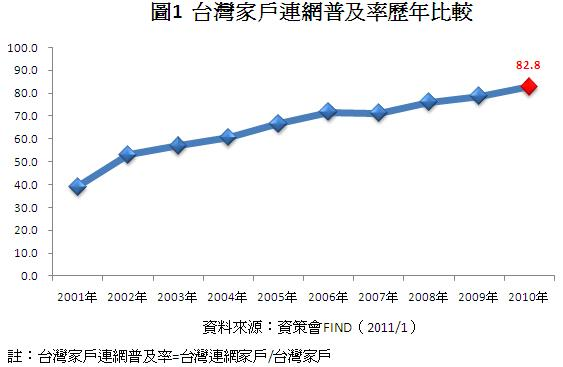
\includegraphics[%
  width=13cm,keepaspectratio]{images/yuwei_2011020901}
\caption{\label{fig:yuwei_2011020901}台灣家戶連網普及率}
%(資料來源:資策會FIND)
\end{figure}

從調查數據如表 \ref{tab:yuwei_2011122005}所示可以發現兩個趨勢:首先,上網民眾的網路活動更加活躍,在上傳與下載檔案、從事線上影音等活動,都有相當顯著的成長,其次,民眾使用網路交易的比例倍增,顯示民眾對於網路的虛擬購物環境,已有相當程度的信任。\cite{資策會FIND}

\begin{table}[H]
\caption{2011/12 月曾上網者之連網使用行為}
\label{tab:yuwei_2011122005}
\renewcommand{\arraystretch}{1.2} % 將表格行間距加大為原來的 1.2 倍
\arrayrulewidth=1pt               % 調整線條粗細為 1pt
\tabcolsep=24pt                   % 調整欄間距為 24pt
%\begin{document}
\begin{tabular}[t]{lll}  % 第一欄位使用 sans serif 字族
\hline
 類別& 各項網路活動 & 2011年(% ) \\
\hline
資訊        & 上傳、下載檔案 & 76.3\\
資訊        & 使用電子化政府服務 & 31.0 \\
溝通        & 傳送即時通訊  & 64.6 \\
溝通        & 擁有個人社交網路  &63.7\\
溝通        & 使用網路電話  & 37.2 \\
溝通              & 網路論壇  & 35.6 \\
娛樂               & 玩線上遊戲  & 55.5 \\
娛樂               & 從事線上影音視訊活動  & 60.2 \\
金融交易               & 網路拍賣或網路購物  & 54.4 \\
金融交易               &利用轉帳或信用卡刷卡繳交帳單   & 29.3 \\
金融交易              &從事實際線上投資理財之交易行為  & 20.4 \\
學習               & 付費線上學習  & 8.1 \\
\hline
\end{tabular}
\end{table}


%\begin{figure}[htbp]
%\centering 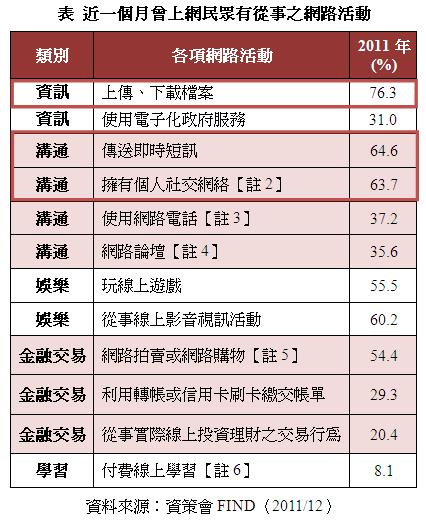
\includegraphics[%
 % width=13cm,keepaspectratio]{images/yuwei_2011122005}
%\caption{\label{fig:yuwei_2011022005}2011/12月曾上網者之連網使用行為}
%(資料來源:資策會FIND)
%\end{figure}

根據以上資料可以了解到近年來網路發展迅速因此消費者習慣也開始改變紛紛改用網路購物因此所謂的『宅經濟』的興起。宅經濟又稱為『閒人經濟』是指不用出門在家就可以從事經濟活動。
根據圖~\ref{fig:Onlinetrends}臺灣線上購物的市場規模自 2006 年 開始到現今每年 二位數的成長趨勢,2010 年市場規模為 3,583 億元,比 2009 年成長了 15%;預估 2011 年線上購物的市場規模可達到 4,300 億元\cite{資策會FIND}。他是個成長非常迅速的市場。

\begin{figure}[htbp]
\centering 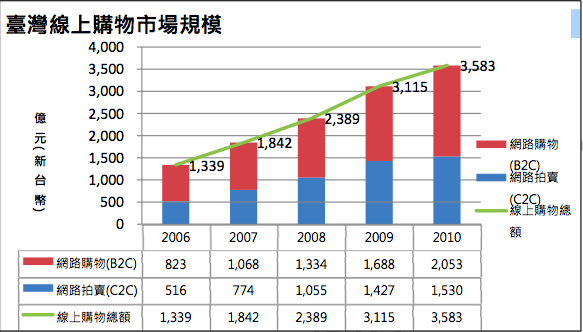
\includegraphics[%
  width=13cm,keepaspectratio]{images/Onlinetrends}
\caption{\label{fig:Onlinetrends}資策會 MIC,2010 台灣線上購物市場規模 3,583 億元,(2012 年 6 月),}
%(資料來源:資策會FIND)
\end{figure}

在近年來網路社交興起,公司紛紛採取社群網站來提升公司的知名度或來作公司產品行銷因此近年產生出新的詞『社群媒體行銷』,觀察網友在最近很火紅的Facebook使用行為上,發現網友使用Facebook的平均使用時間高達439.5分鐘,平均下來,每天約黏在Facebook上面14.65分鐘,已佔了使用社群網站時間的56.6%(資策會FIND)根據互動行銷機構 Rosetta 調查顯示,全球百大零售商已經有 59%在 Facebook 擁有官方粉絲專頁簡稱粉絲團(羅之盈,2010),由此可見,企業也以觀察到Facebook也是一個強大的行銷手法工具之一,透過粉絲專業可以發展出全新的消費者市場,透過Facebook互通性來迅速散播公司相關資訊與雙向溝通可把從粉絲專頁中的人導入公司網路消費者逐群。

但是因為網路通路與實體通路不同的地方是,網路通路所販售的所有商品並不像實體通路有專人解說介紹商品,網路上的消費者只能透過網頁瀏覽器(Web)來觀看網頁上所想購買的商品並沒辦法隨時有像實體通路有專人銷售員介紹的每項功能或使用方法,企業也無法有效掌握顧客的所有需求與企業消費者對商品的滿意度,所以更難推測出未來顧客的消費者行為。



\section{研究目的}
本研究目的是在瞭解透過網路多媒體行銷後的廠商,在網路品牌聲望與品牌知覺是否會影響消費者行為進行分析與推測,提供企業在網路多媒體行銷方面提供有效的建議可以透過本研究更瞭解網路消費者所需求與提升未來企業經營網路虛擬通路之參考


\section{研究流程}

 本研究之流程如圖所示,步驟如下:

1.確定研究動機與範圍

         本研究目的主要目的要探討品牌知覺、品牌聲望、與網路消費者購買行為之關係,研究範圍界定於台灣地區的網路消費者在網路購物中於鈦鍺時尚精品之交易行為。

2-1.文獻收集與研讀

        瞭解本研究的界定主範圍後,開始收集品牌知覺、品牌聲望、網路消費者購買行為、鈦鍺時尚精品等相關文獻,作為研究的基本理論。

2-2. 進行實地訪談

        為了瞭解本研究的鈦鍺時尚精品,相關公司所遇到的問題與消費者行為,前往La Jolla 樂活雅 鈦鍺精品公司實地訪談。

3-1.發展問卷架構

       本研究經過文獻資料與整理及研究探討之後,根據文獻資料與本研究的方向,建立其問卷研發與架構及研究變數,再來針對各個本研究的變數建立研究假設與操作性定義。

3-2.客群分析與訪查

      經過實地親自探訪收集La Jolla 樂活雅 鈦鍺精品公司,所得知的相關客群資料後開始客群分析與訪查本研究相關資料。

4.問卷制作與發放

      本研究方式是採用發放問卷的研究方式,對研究對象進行相關資料的調查;根據研究資料與本研究主題下去研究設計製做問卷,依據本研究該需要的變數去設計選題,即可以開始發放本研究正式的調查問卷,其問卷為網際網路發放方式為收集為主,研究流程如圖~\ref{fig:NPC12}所示。

5.問卷整理與數據分析

      首先針對本研究收回的問卷樣本作敘述性統計分析,了解問卷樣本的基本特性。

6.結論與探討

     依據本研究分析後研究出的結果,統整成文後作研究結論與探討,以作為後續與本文相關研究學者與人員參考之文獻。

\begin{figure}[h]
\centering 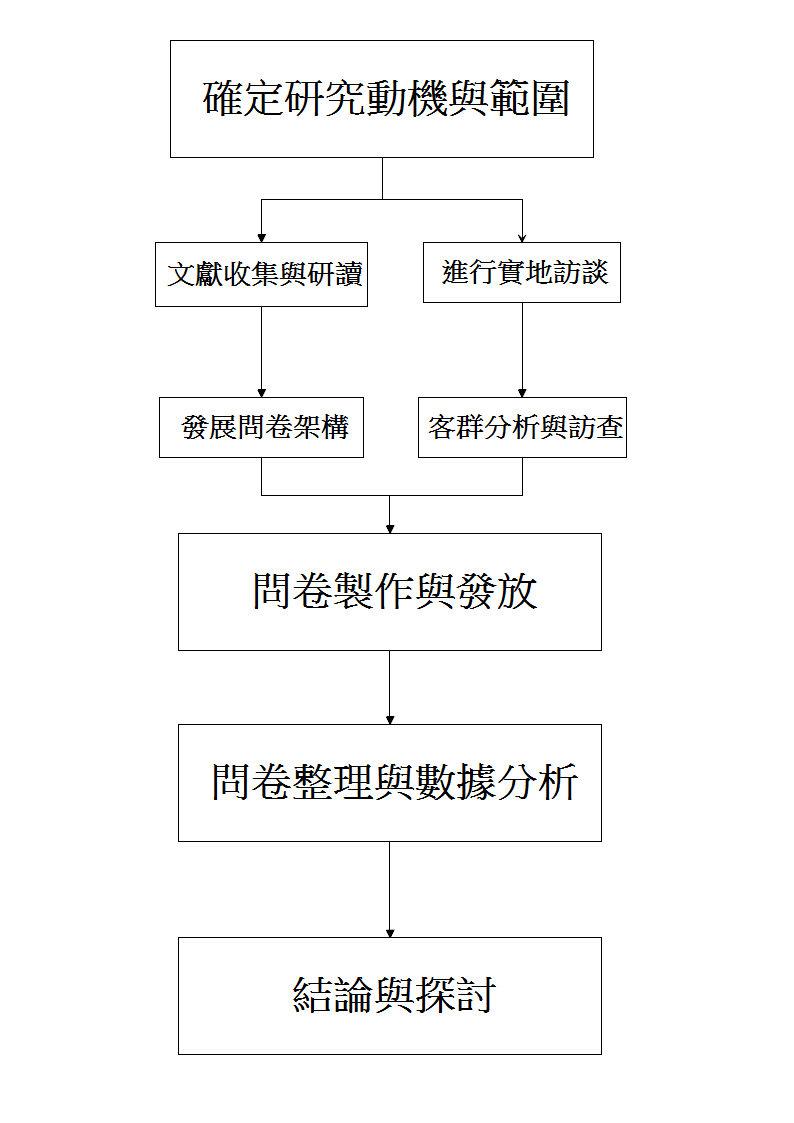
\includegraphics[%
  width=12cm,keepaspectratio]{images/NPC12}
\caption{\label{fig:NPC12}研究流程}
%(資料來源:本研究整理)
\end{figure}



%\section{研究架構}


%\chapter{文獻探討}
%\section{NFC}
%\section{理性行為理論}
%\section{科技接受模式}
%\section{便利性}
%\section{系統品質}
%\section{認知安全性}
%\section{相容性}
%\section{社會影響力}
%
%\chapter{研究設計與方法}
%\section{研究架構}
%\section{研究假說}
%\section{研究構面之操作型定義與衡量問項}
%\section{研究對象}
%\section{資料分析}
%
%\chapter{資料分析與實證研究}
%
%\section{敘述統計分析}
%\section{信度分析}
%\section{建構效度}
%\section{相關分析}
%\section{迴歸分析}
%
%\chapter{研究結論與建議}
%
%\section{研究結論}
%\section{研究貢獻}
%\section{後續研究之建議}
%
